% AUTO-GENERATED durch diagram_generator (REV 7.6, TikZ-Heatmap)
\begin{figure}[!htbp]
\centering
\resizebox{\textwidth}{!}{%
\begin{tikzpicture}
\begin{axis}[
    width=0.7800\textwidth,
    height=0.4000\textheight,
    scale only axis,
    title={Heatmap: Lookup-Latenz p50 (ns/op) (Suchalgorithmus x Workload)},
    xlabel={Workload},
    ylabel={Suchalgorithmus},
    grid=both,
    enlargelimits=0.05,
    view={0}{90},
    colorbar,
    colormap/viridis,
    mesh/cols=6,
    xtick={0,1,...,5},
    ytick={0,1,...,1},
    xticklabels={ycsb\_a,ycsb\_b,ycsb\_c,ycsb\_d,ycsb\_e,ycsb\_f},
    x tick label style={rotate=45,anchor=east,font=\tiny},
    yticklabels={interpolation,k\_ary},
    y tick label style={font=\tiny},
]
\addplot3[matrix plot*, point meta=explicit] coordinates {
    (0,0,2140.0000) [2140.0000]
    (1,0,2050.0000) [2050.0000]
    (2,0,1770.0000) [1770.0000]
    (3,0,5780.0000) [5780.0000]
    (4,0,0.0000) [0.0000]
    (5,0,1870.0000) [1870.0000]
    (0,1,1940.0000) [1940.0000]
    (1,1,2000.0000) [2000.0000]
    (2,1,1961.0000) [1961.0000]
    (3,1,4560.0000) [4560.0000]
    (4,1,0.0000) [0.0000]
    (5,1,2060.0000) [2060.0000]
};
\end{axis}
\end{tikzpicture}
}%
\caption{Heatmap: Lookup-Latenz p50 (ns/op) (Suchalgorithmus x Workload)}
\end{figure}
